%%%%%%%%%%%%%%%%%%%%%%%%%%%%%%%%%%%
%This is the LaTeX ARTICLE template for RSC journals
%Copyright The Royal Society of Chemistry 2016
%%%%%%%%%%%%%%%%%%%%%%%%%%%%%%%%%%%

\documentclass[twoside,twocolumn,9pt]{article}
\usepackage{extsizes}
\usepackage[super,sort&compress,comma]{natbib} 
\usepackage[version=3]{mhchem}
\usepackage[left=1.5cm, right=1.5cm, top=1.785cm, bottom=2.0cm]{geometry}
\usepackage{balance}
\usepackage{times,mathptmx}
\usepackage{sectsty}
\usepackage{graphicx} 
\usepackage{lastpage}
\usepackage[format=plain,justification=justified,singlelinecheck=false,font={stretch=1.125,small,sf},labelfont=bf,labelsep=space]{caption}
\usepackage{float}
\usepackage{fancyhdr}
\usepackage{fnpos}
\usepackage[english]{babel}
\addto{\captionsenglish}{%
  \renewcommand{\refname}{Notes and references}
}
\usepackage{array}
\usepackage{droidsans}
\usepackage{charter}
\usepackage[T1]{fontenc}
\usepackage[usenames,dvipsnames]{xcolor}
\usepackage{setspace}
\usepackage[compact]{titlesec}
\usepackage{hyperref}
%%%Please don't disable any packages in the preamble, as this may cause the template to display incorrectly.%%%
% \usepackage{epstopdf}%This line makes .eps figures into .pdf - please comment out if not required.

\definecolor{cream}{RGB}{222,217,201}

\usepackage[utf8]{inputenc}
\usepackage{xargs}                      % Use more than one optional parameter in a new commands (newcommandx)
% \usepackage{hyperref}                   % Must *always* come before cleveref.
\usepackage[capitalize]{cleveref}
\usepackage[colorinlistoftodos,prependcaption,textsize=tiny]{todonotes} % add 'disable' to optional args to turn off.
\usepackage{booktabs}
\usepackage{subcaption}
\usepackage{listings}
\usepackage{caption}
\usepackage{multirow}

\Crefname{figure}{Figure}{Figures}
\crefname{figure}{Fig.}{Figs.}
\Crefname{section}{Section}{Sections}
\crefname{section}{§}{§§}
\newcommand{\rfig}[1]{Fig. \ref{#1}}


\definecolor{purple}{RGB}{75,0,130}
\definecolor{neonyellow}{RGB}{244, 238,66}
\definecolor{cream}{RGB}{222,217,201}

\newcommandx{\jason}[2][1=]{\todo[linecolor=red,backgroundcolor=green!25,bordercolor=red,#1]{#2}}
\newcommandx{\jasoni}[2][1=]{\todo[linecolor=red,backgroundcolor=green!25,bordercolor=red,inline,#1]{#2}}
\newcommandx{\tyson}[2][1=]{\todo[linecolor=green,backgroundcolor=orange!25,bordercolor=blue,#1]{#2}}
\newcommandx{\tysoni}[2][1=]{\todo[linecolor=green,backgroundcolor=orange!25,bordercolor=blue,inline,#1]{#2}}
\newcommandx{\philip}[2][1=]{\todo[linecolor=yellow, backgroundcolor=yellow!25,bordercolor=orange,#1]{#2}}
\newcommandx{\philipi}[2][1=]{\todo[linecolor=yellow, backgroundcolor=yellow!25,bordercolor=orange,inline,#1]{#2}}
\newcommandx{\autarchi}[2][1=]{\todo[linecolor=yellow, backgroundcolor=yellow!25,bordercolor=orange,inline,#1]{#2}}
\newcommandx{\grover}[2][1=]{\todo[linecolor=blue,backgroundcolor=yellow!25,bordercolor=blue,#1]{#2}}
\newcommandx{\groveri}[2][1=]{\todo[linecolor=blue,backgroundcolor=yellow!25,bordercolor=blue,inline,#1]{#2}}
\newcommandx{\brian}[2][1=]{\todo[linecolor=purple,backgroundcolor=neonyellow!25,bordercolor=purple,inline,#1]{#2}}
\newcommandx{\briani}[2][1=]{\todo[linecolor=purple,backgroundcolor=neonyellow!25,bordercolor=purple,inline,#1]{#2}}

\newcommand{\bs}{BioScript}
\newcommand{\tool}{\textbf{\textcolor{red}{AquaFlow}}}


%Pretty code printing.
\lstset{
	float,
   	basicstyle=\footnotesize\ttfamily,
    xleftmargin=2em,
    framexleftmargin=1.5em,
    numbers=left,
    stepnumber=1,
    showstringspaces=false,
    tabsize=1,
    breaklines=true,
    breakatwhitespace=false,
    keywordstyle=\color{blue},
    morekeywords={mix, split, heat, detect, save, repeat, times, while, if, else, elseif, with, at, of, on, for, components, netlist, dispense, dispose, instructions, manifest},
}

\begin{document}

\pagestyle{fancy}
\thispagestyle{plain}
\fancypagestyle{plain}{

%%%HEADER%%%
\fancyhead[C]{
\includegraphics[width=18.5cm]{assets/header_bar}}
\fancyhead[L]{\hspace{0cm}\vspace{1.5cm}
\includegraphics[height=30pt]{assets/journal_name}}
\fancyhead[R]{\hspace{0cm}\vspace{1.7cm}
\includegraphics[height=55pt]{assets/RSC_LOGO_CMYK}}
\renewcommand{\headrulewidth}{0pt}
}
%%%END OF HEADER%%%

%%%PAGE SETUP - Please do not change any commands within this section%%%
\makeFNbottom
\makeatletter
\renewcommand\LARGE{\@setfontsize\LARGE{15pt}{17}}
\renewcommand\Large{\@setfontsize\Large{12pt}{14}}
\renewcommand\large{\@setfontsize\large{10pt}{12}}
\renewcommand\footnotesize{\@setfontsize\footnotesize{7pt}{10}}
\makeatother

\renewcommand{\thefootnote}{\fnsymbol{footnote}}
\renewcommand\footnoterule{\vspace*{1pt}% 
\color{cream}\hrule width 3.5in height 0.4pt \color{black}\vspace*{5pt}} 
\setcounter{secnumdepth}{5}

\makeatletter 
\renewcommand\@biblabel[1]{#1}            
\renewcommand\@makefntext[1]% 
{\noindent\makebox[0pt][r]{\@thefnmark\,}#1}
\makeatother 
\renewcommand{\figurename}{\small{Fig.}~}
\sectionfont{\sffamily\Large}
\subsectionfont{\normalsize}
\subsubsectionfont{\bf}
\setstretch{1.125} %In particular, please do not alter this line.
\setlength{\skip\footins}{0.8cm}
\setlength{\footnotesep}{0.25cm}
\setlength{\jot}{10pt}
\titlespacing*{\section}{0pt}{4pt}{4pt}
\titlespacing*{\subsection}{0pt}{15pt}{1pt}
%%%END OF PAGE SETUP%%%

%%%FOOTER%%%
\fancyfoot{}
\fancyfoot[LO,RE]{\vspace{-7.1pt}
\includegraphics[height=9pt]{assets/LF}}
\fancyfoot[CO]{\vspace{-7.1pt}\hspace{13.2cm}
\includegraphics{assets/RF}}
\fancyfoot[CE]{\vspace{-7.2pt}\hspace{-14.2cm}
\includegraphics{assets/RF}}
\fancyfoot[RO]{\footnotesize{\sffamily{1--\pageref{LastPage} ~\textbar  \hspace{2pt}\thepage}}}
\fancyfoot[LE]{\footnotesize{\sffamily{\thepage~\textbar\hspace{3.45cm} 1--\pageref{LastPage}}}}
\fancyhead{}
\renewcommand{\headrulewidth}{0pt} 
\renewcommand{\footrulewidth}{0pt}
\setlength{\arrayrulewidth}{1pt}
\setlength{\columnsep}{6.5mm}
\setlength\bibsep{1pt}
%%%END OF FOOTER%%%

%%%FIGURE SETUP - please do not change any commands within this section%%%
\makeatletter 
\newlength{\figrulesep} 
\setlength{\figrulesep}{0.5\textfloatsep} 

\newcommand{\topfigrule}{\vspace*{-1pt}% 
\noindent{\color{cream}\rule[-\figrulesep]{\columnwidth}{1.5pt}} }

\newcommand{\botfigrule}{\vspace*{-2pt}% 
\noindent{\color{cream}\rule[\figrulesep]{\columnwidth}{1.5pt}} }

\newcommand{\dblfigrule}{\vspace*{-1pt}% 
\noindent{\color{cream}\rule[-\figrulesep]{\textwidth}{1.5pt}} }

\makeatother
%%%END OF FIGURE SETUP%%%


%%%TITLE, AUTHORS AND ABSTRACT%%%
\twocolumn[
  \begin{@twocolumnfalse}
\vspace{3cm}
\sffamily
\begin{tabular}{m{4.5cm} p{13.5cm} }


\includegraphics{assets/DOI} & \noindent\LARGE{\textbf{Fabricating Microfluidic Devices from High-Level Languages$^\dag$}} \\%Article title goes here instead of the text "This is the title"
\vspace{0.3cm} & \vspace{0.3cm} \\

 & \noindent\large{Jason Ott, Tyson Loveless, Daniel Tan, Heran Bhakta, Brian Crites, Jeffrey McDaniel, William Grover, and Philip Brisk} \\%Author names go here instead of "Full name", etc.


\includegraphics{assets/dates} & \noindent\normalsize{
    Designing, fabricating, and testing microfluidic laboratory-on-a-chip (LoC) devices is an complex task requiring collaboration from biologists, chemists, engineers, and computer scientists --- 
a time-intensive and human-resource-expensive process for small devices promising large time- and cost-saving benefits.
In this paper, we introduce an automated system capable of fabricating LoC devices from a domain specific language.
The workflow expedites the development of new chips while simultaneously allowing for far greater complexity of microfluidic devices than currently tenable.
} \\%The abstract goes here instead of the text "The abstract should be..."

\end{tabular}

 \end{@twocolumnfalse} \vspace{0.6cm}

  ]

%%%END OF TITLE, AUTHORS AND ABSTRACT%%%

%%%FONT SETUP - please do not change any commands within this section
\renewcommand*\rmdefault{bch}\normalfont\upshape
\rmfamily
\section*{}
\vspace{-1cm}

%%%FOOTNOTES%%%

\footnotetext{University of California, Riverside, Riverside, CA, USA.; E-mail: philip@cs.ucr.edu}

%Please use \dag to cite the ESI in the main text of the article.
%If you article does not have ESI please remove the the \dag symbol from the title and the footnotetext below.
\footnotetext{\dag~Electronic Supplementary Information (ESI) available: [details of any supplementary information available should be included here]. See DOI: 10.1039/b000000x/}
%additional addresses can be cited as above using the lower-case letters, c, d, e... If all authors are from the same address, no letter is required

% \footnotetext{\ddag~Additional footnotes to the title and authors can be included \emph{e.g.}\ `Present address:' or `These authors contributed equally to this work' as above using the symbols: \ddag, \textsection, and \P. Please place the appropriate symbol next to the author's name and include a \texttt{\textbackslash footnotetext} entry in the the correct place in the list.}

%%%END OF FOOTNOTES%%%

%%%MAIN TEXT%%%%
%=================================================================================
% Introduction
%=================================================================================
\section{Introduction}
\label{sec:introduction}
Microfluidic Laboratory-on-a-Chip (LoC) devices promise radical transformations for chemistry and biology.
%, a class of powerful devices are capable of radically transforming chemistry and biology.
LoC technology works by miniaturizing laboratory procedures down to the sub-millimeter scale \cite{thorsen02}, by integrating functional components (e.g., dispensing, filters, mixers, detectors) along with fluid handling into a single package.
LoC technologies come in two prominent flavors: flow- and %droplet-based.
discrete-based.
Flow-based LoC devices rely on external pressure to move fluid through the device interacting with the various functional components the device employs.
%Droplet-based 
Discrete-based LoC devices function by manipulating discrete droplets of fluid, either in immiscible phases with low Reynolds number and laminar flow regimes, or on a 2D electrical grid. %on a 2D electrical grid.
The advent and improvement of microfluidic devices over the last two decades has heralded the promise of radical transformation ``within 5 years,'' \footnote{This isn't a literal 5 years, it's euphemistic for a technological break-thru that is constantly just out of reach, but \textit{will eventually} fundamentally transform the field, e.g. nuclear fission is perpetually 10 years from being ready.} which has yet to be realized.
With current technological limitations, only the use of tools, engineered to help aid in the design and fabrication of devices will get us there.
%flow-based microfluidic devices demonstrate the strongest potential for delivering on the promised transformations first.

The perpetual ``5 year'' promise is a result of the myriad of moving parts required for developing a technology that is simple, adoptable, and reproducible.
Historically, the design of flow-based LoC devices has been by hand, using CAD tools to draw a device and before fabricating using one of the myriad of fabrication techniques available --- %fabricating the device using any one of the myriad of fabrication techniques.
a laborious task requiring significant investment from the scientist for even the simplest of devices.

This paper introduces \tool{}, a toolchain aiming to provide tangible progress aimed at reducing the ``5 year'' perpetuity claim by making it easier to express and design flow-based microfluidic devices.
\tool{} borrows concepts native to Computer Science: programming languages, compiler theory, and architectural synthesis techniques, and applies them to the design, synthesis, and execution of flow-based microfluidic devices.
\tool{} extends the Domain Specific Language (DSL) presented in Ott et al's work\cite{ott2018bioscript} to emit a netlist\cite{mcdaniel2015flow} of components and their connections that McDaniel et al's work\cite{McDaniel2013} is capable of understanding.  Finally, Ott et al's work \cite{ott2018bioscript} is further extended to generate the valve actuation sequences necessary to power active-flow-based microfluidic LoCs.
% \tool{} is capable of accepting a high level specification expressed in \cite{ott2018bioscript}, 

%=================================================================================
% Background
%=================================================================================
\subsection{Background}
\label{sec:background}

%=================================================================================
% Programming languages for Microfluidics
%=================================================================================
\subsubsection{Programming Languages for Microfluidics}
The past several years has seen an increased interest in programming languages design targeting microfluidic devices.

\textbf{\textit{BioStream}} targets a programmable LoC whose primary purpose focuses upon serial dilution protocols coupled with fluidic mixers \cite{urbanski06, ThiesMINMIX}.
\textit{BioStream}'s abstractions allows users to specify target concentrations%.Those concentrations would be the 
as input to automatically generate serial dilution protocols.
Although 
\textit{BioStream} %is restricted to a single form and function and cannot serve as a general purpose microfluidic programming language.
allows for high level abstractions for basic microfluidic protocols, it did not support general purpose programmability, and its specification and compiler was never release after publication.

\textbf{\textit{Aquacore Instruction Set} (AIS)}\cite{amin_isca07, amin13} allows a scientist to program a microvalve-based LoC supporting several components traditionally found in laboratory settings.
This language is specific to only the AquaCore LoC devices and cannot be used outside the context of said devices.
AIS closely resembles \textit{assembly language}, an esoteric and enigmatic language exposing hardware-level details of the computer architecture requiring considerable expertise to work with.
Although powerful, the need for expertise renders AIS an unlikely candidate for adoption from scientists wishing to quickly and efficiently design and synthesize LoCs --- indeed, computer scientists have spent decades building abstractions reducing the need to write in assembly language almost entirely, as the language complexity bottlenecks the functional process.

\textbf{\textit{BioCoder}} began as an ontology \cite{Thies_BioCoder} to describe assays in a unified format.
It was later extended to target digital microfluidic biochips\cite{McDaniel2013, Grissom_JetC, CURTIS_BIOCODER, curtis2018compiler} (DMFBs).
\textit{BioCoder} is an interesting proof-of-concept, however, much like \textit{AIS} is arcane and unfriendly.
\textit{BioCoder}, unlike \textit{AIS}, is a general purpose language targeting microfluidic devices, although it is restricted to targeting a DMFB simulator\cite{grissom2015open}.

\textbf{\textit{Puddle}}\cite{willsey2019puddle}, a DSL embedded in the Python programming language, utilizes an Application Programming Interface (API) to manipulate droplets on a DMFB device.
In general, the language is not re-targetable, meaning it only execute on \textit{Puddle}'s own hardware; and is unable to support flow-based devices.
However, it provides powerful video sensors to monitor fidelity during execution, track droplet volume, and identify malfunctioning areas on the device, preventing further use.

\textbf{\textit{\bs{}}}\cite{ott2018bioscript} is a DSL replete with a fluidic-based type system
\footnote{A type system is a component of a programming language ensuring a user creates a valid program, e.g., prevent a user from: $x="a" + 2$} 
designed to allow for easy assay creation while maintaining a safe execution environment.
\textit{\bs{}} abstracts many of the complexities present in \textit{AIS} and \textit{BioCoder} away in order to help scientists efficiently develop complicated assays in a succinct form; mimicking what computer scientists have done with respect to assembly language. When published, \bs{} was only capable of targeting several open-source DMFB devices. We extend \bs{} in this paper to target the automated-fabrication of continuous-flow LoC devices.

%=================================================================================
% Compilation
%=================================================================================
\subsubsection{Compilation}
\label{sec:compilation}
The role of a compiler is to take high-level instructions, typically in the form of a programming language (e.g., Python or C++), and translate them into sets of low-level \textit{machine code} --- instructions a physical architecture is capable of understanding.
This process is illustrated in \cref{fig:compilation_process}, 
in which a user provides an input program, written in C++ or Java in this case, and the compiler translates the input into an \textit{Intermediate Representation} (IR), and then generates the machine code that is specific to the processor on which the program will execute.
The translation into IR might seem unnecessary; however, if it didn't exist, there would need to be a mapping from each language to the specific processor architecture.
In other words, the translation to an IR introduces a common denominator that allows computer scientists
\footnote{Wishful thinking, of course, the ``one compiler to rule them all'' only exists as an ideal.}
to build one compiler that is capable of accepting any language as input and is capable of targeting any processor architecture.
IR also allows a myriad of standardized optimizations (not depicted) to the input code that typically reduces execution time and better utilizes computational resources.
Once optimizations occur, the compiler can translate the IR code into the machine code for the processor architecture(s) desired for execution.

Applying traditional computer science techniques, such as compilers, to digital microfluidic architectures and design is an active area of research \cite{curtis2018compiler,ott2018bioscript,grissom2015open}; however, there are no known applications of traditional computer science techniques combining programming languages and compilers to target flow-based microfluidic architectures.

\begin{figure*}
    % \begin{subfigure}{0.45\textwidth}
    %     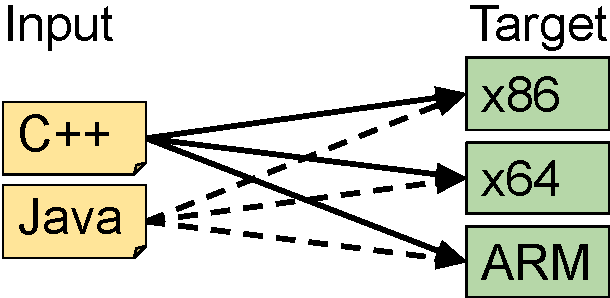
\includegraphics[width=0.8\textwidth]{figures/compilation_process_without_ir.pdf}
    %     \caption[short]{}
    %     \label{fig:compilation_process_no_ir}
    % \end{subfigure}\hfill%
    % This aligns the subfigures on one line.
    % \begin{subfigure}{0.55\textwidth}
        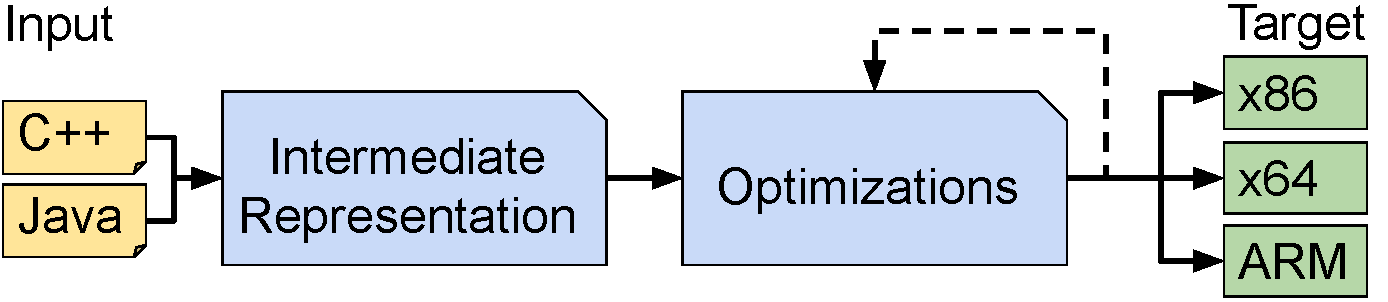
\includegraphics[width=\textwidth]{figures/compilation_process_with_ir.pdf}
        % \caption[short]{}
        % \label{fig:compilation_process_ir}
    % \end{subfigure}
    \caption{The job of a compiler: converting an input language (C++, Java) to machine code a specific architecture (x86, x64, ARM) can execute.  The dotted line denotes a self-loop the compiler employs for its various optimizations it runs.}
    \label{fig:compilation_process}
\end{figure*}

%=================================================================================
% Architectural Synthesis
%=================================================================================
\subsubsection{Architectural Synthesis}
\label{sec:synthesis}

Architectural synthesis is the automatic mapping of a high-level description to its corresponding low-level implementation.
It serves as an abstraction allowing the design and creation of complex architectures that might be untenable to create while simultaneously lowering the domain-specific knowledge a user must employ.
In traditional architectural synthesis, a designer writes a specification in a language like Verilog or VHDL\footnote{Very High Speed Integrated Circuit (VHSIC) Hardware Description Language (VHDL)} to describe how the device should operate.
The specification comes in the form of netlists --- each component has connections between itself and some set of other components.
This specification is then sent to a synthesis engine which attempts to place and route the components with their connections, as prescribed by the netlists.
Placement and routing is constrained by the specification (e.g., signal timing, space, or component size): two components must reside near enough to each other or the signal will not travel between the components within the specified clock-cycle, ruining the computation.
After the successful synthesis of the design the device is sent for fabrication.

In hardware design, architectural synthesis began with designers placing and routing discrete gates (components) by hand; placing an \textsf{XOR} or \textsf{NAND} gate and connecting their inputs and outputs by hand\jason{cite?}.
Shortly thereafter, designers created more complex components by combining groups of discrete gates into one larger, more complex component.
Thus, instead of placing a series of \textsf{NAND} gates, they would place a full-adder\footnote{a component capable of doing basic arithmetic.}.
This simple grouping quickly increased the complexity and capabilities of both the designers and their fabricated devices.
% This abstraction is, in principle, currently employed by hardware architects today.

In hardware architecture, the mapping between components and their low-level implementations are mature. In many hardware design architectures, component selection is straightforward and obvious --- an architect needs to add numbers, so they employ a full adder.
In the fluidic context this mapping isn't so clear; there are numerous constraints that require a priori knowledge that directly impacts the components that are selected for use during execution.
A case not present in the classical context of hardware architecture: a hardware architect need only know that arithmetic will occur, they require no other knowledge -- nothing about the types, size, or quantity of numbers. \jasoni{From Brian: I would specify something more like at the end of the day we only have to care if the electical value is high or low, and everything else is built on top of that single idea whereas with microfulidics the basics are much more complex. In architecture we would care about type (numerics) and size (bithwidth).}
For instance, the length of mixer (by time or by physical size) is dependent upon several properties pertaining to the input fluids, (e.g., viscosity). 
The 3D$\mu$F tool\cite{sanka20193d} has component generators which are capable of meeting architectural needs such as parameterizing the number outputs in a dilution bridge or the length and number of turns in a serpentine mixer. While this easies the burden of creating new components to meet architectural requirements, it still requires a large amount of domain expertise to know what parameters to specify to meet the fluidic needs. To the best of our knowledge there is only one previous work which utilizes user specified parameters describing the fluid properties and the desired dilution to generate a serpentine mixer which can meet those requirements \cite{grimmer2018meander}.


% \Cref{fig:synthesis_process} details the synthesis of a microfluidic device beginning with a high level specification written in \bs. The specification generates a netlist \cref{fig:net_list}, a hierarchical list of connections between components which apply operations to fluids.
% The netlist is generated by parsing the high-level \bs code into a directed acyclic graph (DAG) representing the flow of data through the program, which can be directly translated into the netlist.
% %and then converting the DAG directly into a netlist.
% Each node in the DAG is converted into a component which matches that functionality and the parameters supplied to it by the user (described below), while edges are translated as connections.
% From the netlist, the synthesis workflow aims to place all components on a chip \cref{fig:placement}.
% Once a valid placement is found, the synthesis tool attempts to route pathways between the components defined in the netlist \cref{fig:routing}.
% Assuming placement and routing succeed, the synthesis tool can fabricate the device \cref{fig:fabricated_chip}.

% \briani{consider if we want the above and below sections to be a single section on synthesis?}

%=================================================================================
% Component Generation & Selection
%=================================================================================
% \subsection{Component Generation \& Selection}
% \label{sec:component_selection}
% \tysoni{this section is difficult to read/follow... It seems you don't know what you're trying to say.  As this seems to be background info, state explicitly what has been done while delineating what is the new contribution}

% Continuous-flow microfluidic devices use the geometries of the device's design in order to utilize fluid dynamics to induce some type of desired fluidic outcome. 
% While there may be a direct translation from a function to a component for functions which only take fluidic parameters, components which have additional non-fluidic parameters are more difficult to translate.
% Coupling these non-fluidic parameters which are provided by the user with the fact that components are fixed after fabrication necessitates the ability to generate a component that meets these specific parameters. 
% In order to accomplish this task, we use a combination of pre-created components for non-parameterized functions along with component generators which can generate components to meet the specific parameters provided by the user.
% Since currently the vast majority of continuous-flow microfluidic devices are fully designed by hand, there has been little work in the automatic generation of components based on user specific parameters.
% To our knowledge,  

%=================================================================================
% Fabrication Methods
%=================================================================================
\subsubsection{Fabrication Methods}
\label{sec:fabrication_methods}

The fabrication of flow-based microfluidic devices is a rich research area, with many significant contributions borrowed from traditional computer architecture fabrication.
While this paper doesn't claim any contributions for techniques, we do present 
%this contribution is 
a complete synthesis workflow which is dependent upon existing fabrication techniques.

Flow-based microfluidic devices rely on fluid continuously flowing through networks of components and channels.
These channels and components are patterned onto one or more layers on the device.
Each patterned layer may be imprinted in either a rigid substrate (e.g., acrylic) \cite{el2006cells,hung2005continuous,pamme2007continuous} or a flexible polymer (e.g., \textit{polydimethylsiloxane (PDMS))}\cite{xia1998soft}.
To enclose the patterned layer(s), a rigid non-patterned material (e.g., glass) may be bonded to the topmost patterned layer, preventing contaminants or particulates from reaching internal layers and/or fluids and provide stability for flexible substrates.
To provide I/O access for fluids, small holes are either drilled (rigid material) or punched (flexible material) into the device.

Creating the patterned layer is dependent upon technology.\jason{this is vague...}
In general, there is an inverse relationship between the size of the feature and cost of the fabrication equipment required; however, most biological media (e.g., cells, organisms, etc.) are not suited for arbitrarily small features.
For fabricating rigid substrates, desktop CNC milling\cite{lashkaripour2019performance,lashkaripour2018desktop} is representative of a lower-cost, larger feature-size fabrication method; microfabrication through photolithography is representative of a relatively higher-cost, smaller feature-size fabrication method.
CNC milling cuts channels into polycabonate thermoplastic polymers through the use of a drill bit, whereas microfabrication etches patterns into glass using photolithography.
While a biologist can use any fabrication technique available to them, ensuring compatibility between material and the biological media influences both the material and fabrication technique used for generating a device.

Fabricating devices comprised of flexible materials are both more complex and more expensive than that of a rigid material\cite{xia1998soft}. The most common flexible material used in continuous-flow microfluidics, polydimethylsiloxane (PDMS), is ideal for its durability however, it suffers from being permeable to certain fluids and its fabrication for use as a microfluidic medium requires the construction of a physical rigid mold (as the final design's negative) and the precise mixture of reactants and curing process for success. The curing process requires exposure to air and/or heat to imprint into the mold before being attached to a rigid substrate to cap the stamped fluidic channel and component design. When working with small features, additional steps such as degassing to remove bubbles is also necessary, rending this as both costly and error-prone -- particularly when done by hand.

%production of a physical mold is required for photolithography. For flexible materials, such as PDMS, 
%it must first be in a liquid state so it can be poured onto the mold.
%The liquid then, once exposed to air and/or heat, partially harden to imprint the mold's pattern.
%Once the patterned medium has partially cured, it can then be mounted on a rigid substrate.
%However, this process is complicated by the necessity of additional steps such as degassing to remove bubbles; increasing time and cost of fabrication, and implicitly hindering scalability.

Another fabrication technique, Additive manufacturing (e.g., 3D printing\cite{gong2016high,rogers20153d,waheed20163d}) creates enclosed rigid 3D structures by %not placing any material where a channel should exist.
encapsulating the design within rigid material.
Additive manufacturing removes the need to bond distinct patterned layers; a key advantage over other fabrication techniques.
This advantage, however, comes with 2 costs: 3D printing is opaque, unlike glass or PDMS, which makes the use of fluid imaging almost impossible.
Second, recent research has shown that different 3D printing technologies introduce materials that expose different toxicity levels %and that these levels, in the most extreme cases, 
, though these can be remedied by exposure to ultraviolet light\cite{oskui2015assessing}.

Each of the existing fabrication methods have their strengths and weaknesses; however, they all share a common setback: the requirement of the manual placement of components and routing between them.
This bottleneck demonstrates a clear and present need for an automated tool that handles the synthesis of a device from a high-level language.

\begin{figure*}[htb]
    \centering
    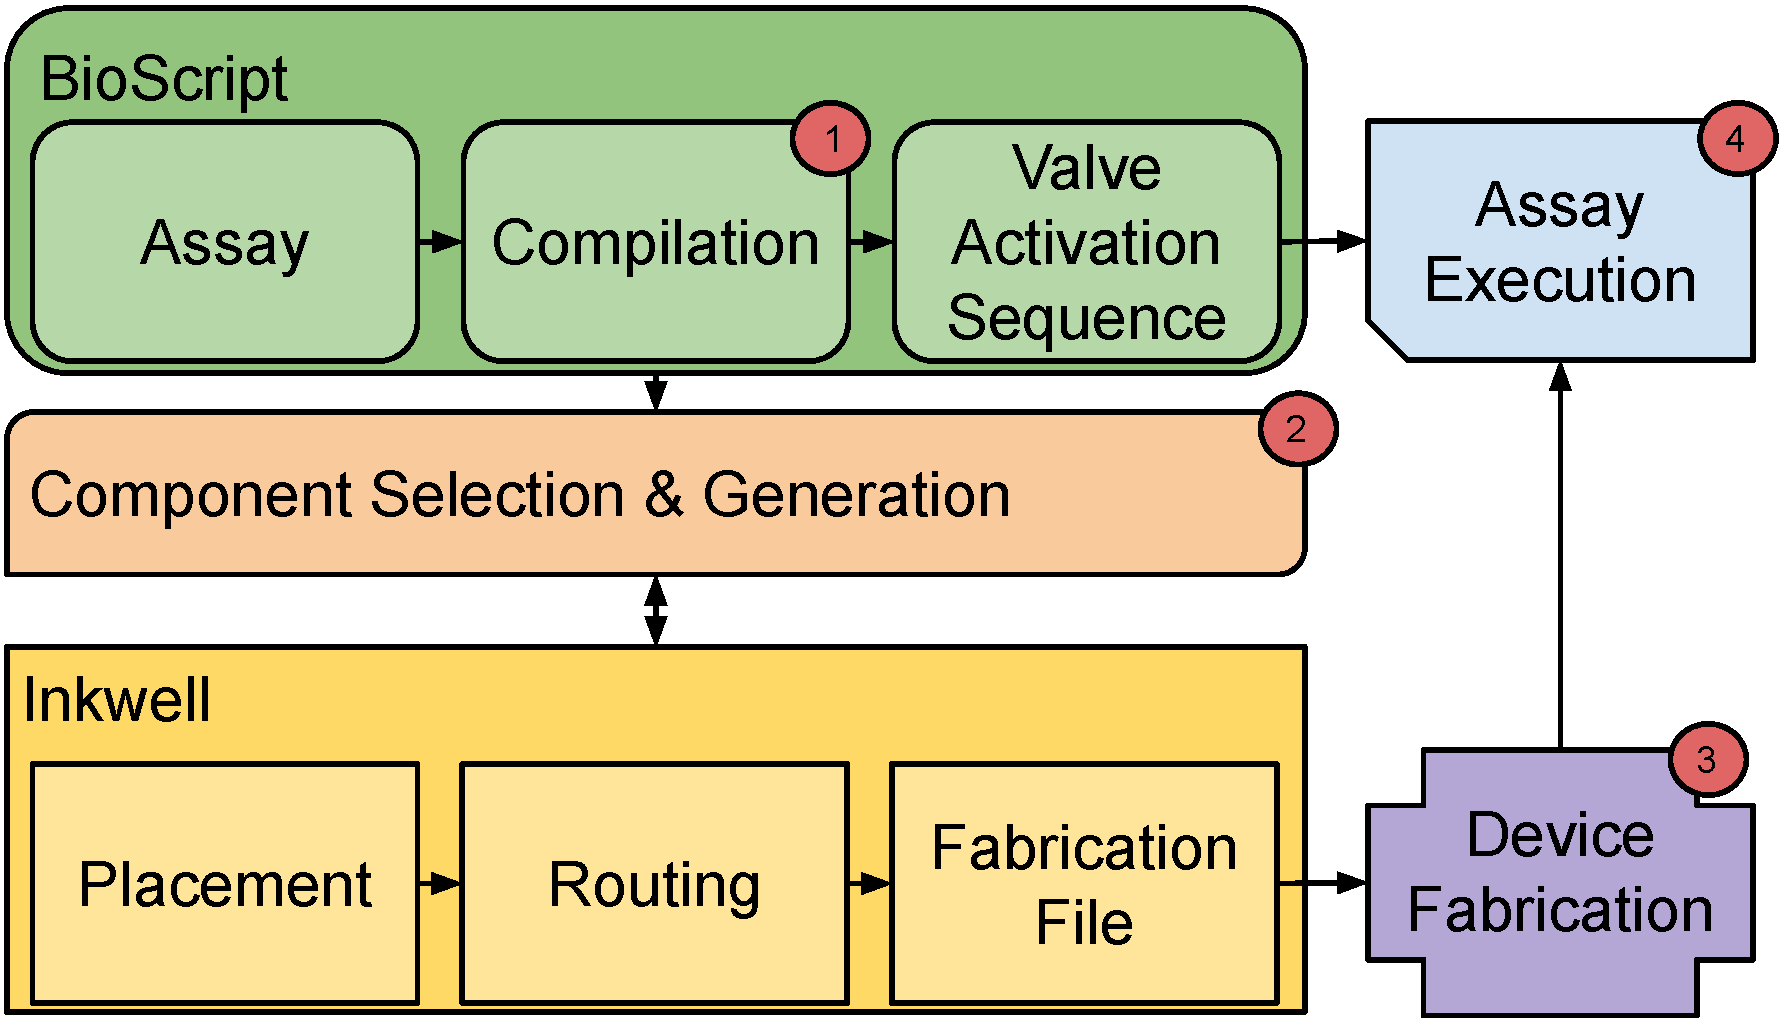
\includegraphics[width=0.8\textwidth]{figures/system_overview.pdf}
    \caption{Overview of the systems\protect{\cite{ott2018bioscript,mcdaniel2018design}} responsible for transforming an assay to the corresponding microfluidic device.}
    \label{fig:workflow}
\end{figure*}



\begin{figure*}[tb]
\centering
    \begin{subfigure}{0.35\textwidth}
        \begin{lstlisting}
manifest "hydrochloric acid"
manifest buffer

instructions:
hcl = dispense "hydrochloric acid"
buf = dispense buffer
dilution = mix hcl with buf
dispose buf
        \end{lstlisting}
        \caption[short]{}
        \label{fig:bs_program}
    \end{subfigure}
    %
    \begin{subfigure}{0.35\textwidth}
        \begin{lstlisting}
components: {
    input_1,
    input_2,
    mixer_1,
    output_1
},
netlist: {
    (input_1, mixer_1),
    (input_2, mixer_1),
    (mixer_1, output_1)
}
        \end{lstlisting}
        \caption[short]{}
        \label{fig:net_list}
    \end{subfigure}
    % Intentional blank line here.
    
    % End intentional blank line.
    \begin{subfigure}{0.33\textwidth}
        \fbox{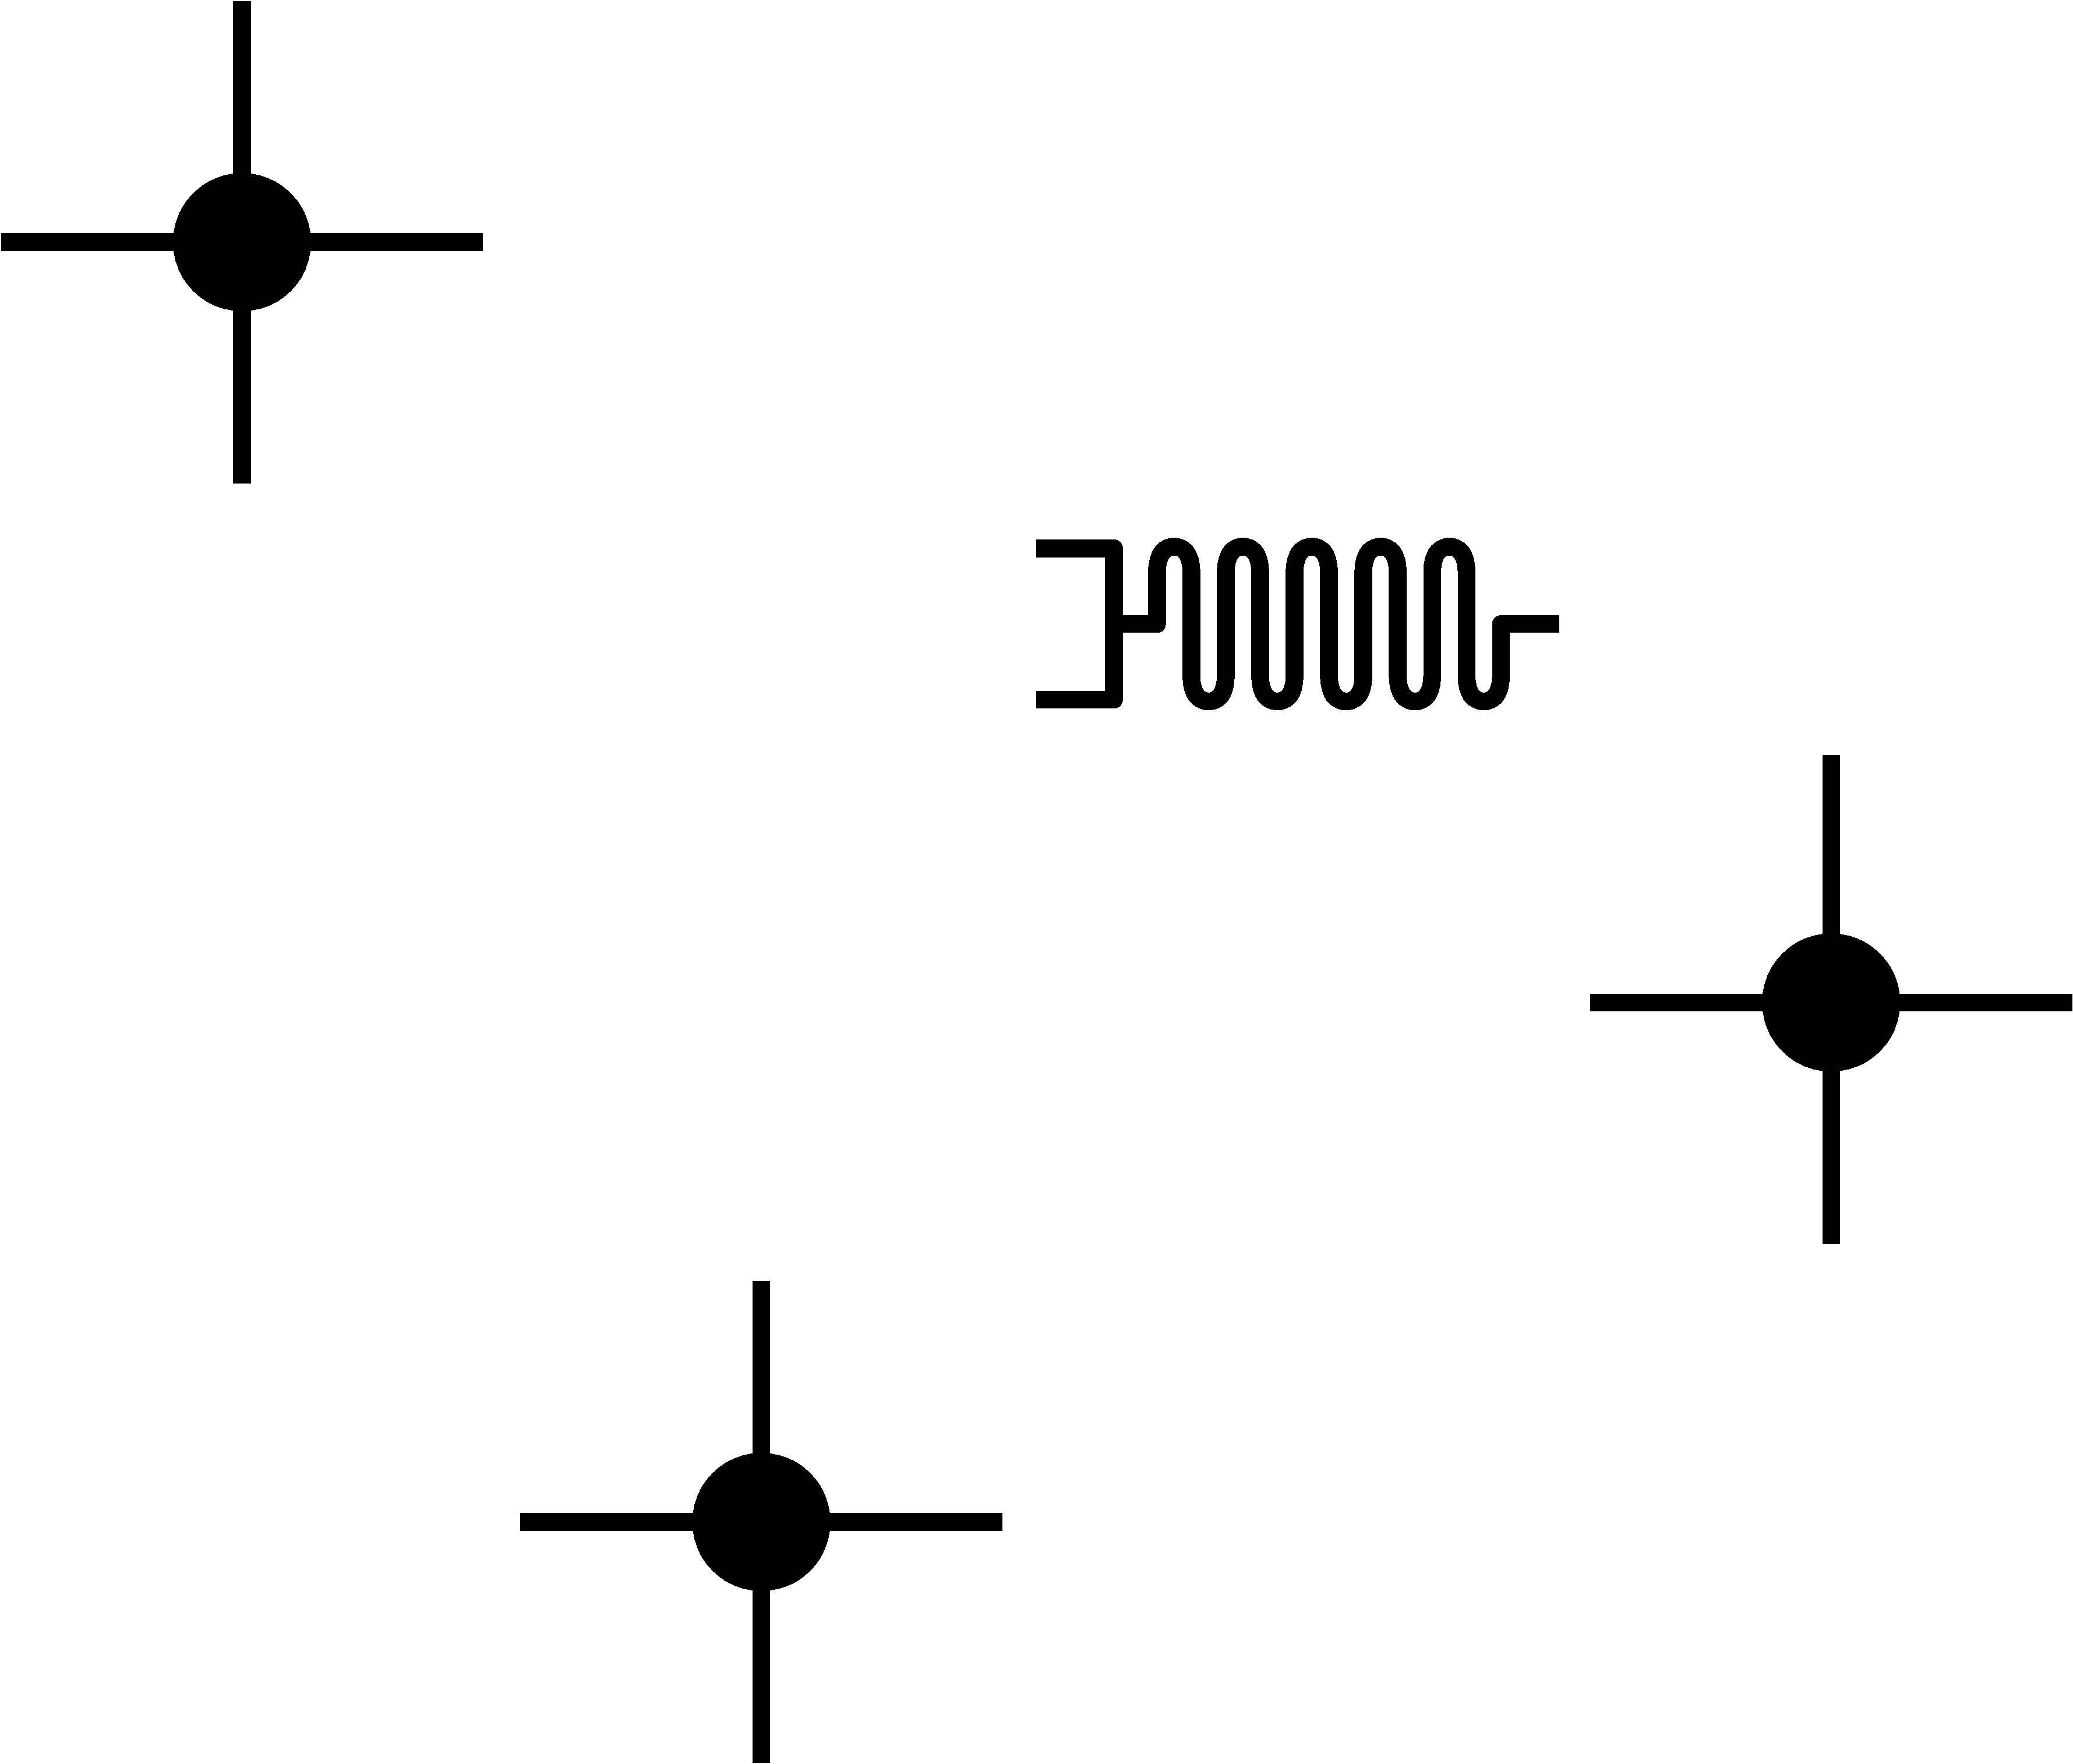
\includegraphics[width=0.9\textwidth]{figures/synthesis_process_placement.pdf}}
        \caption[short]{}
        \label{fig:placement}
    \end{subfigure}
    \begin{subfigure}{0.33\textwidth}
        \fbox{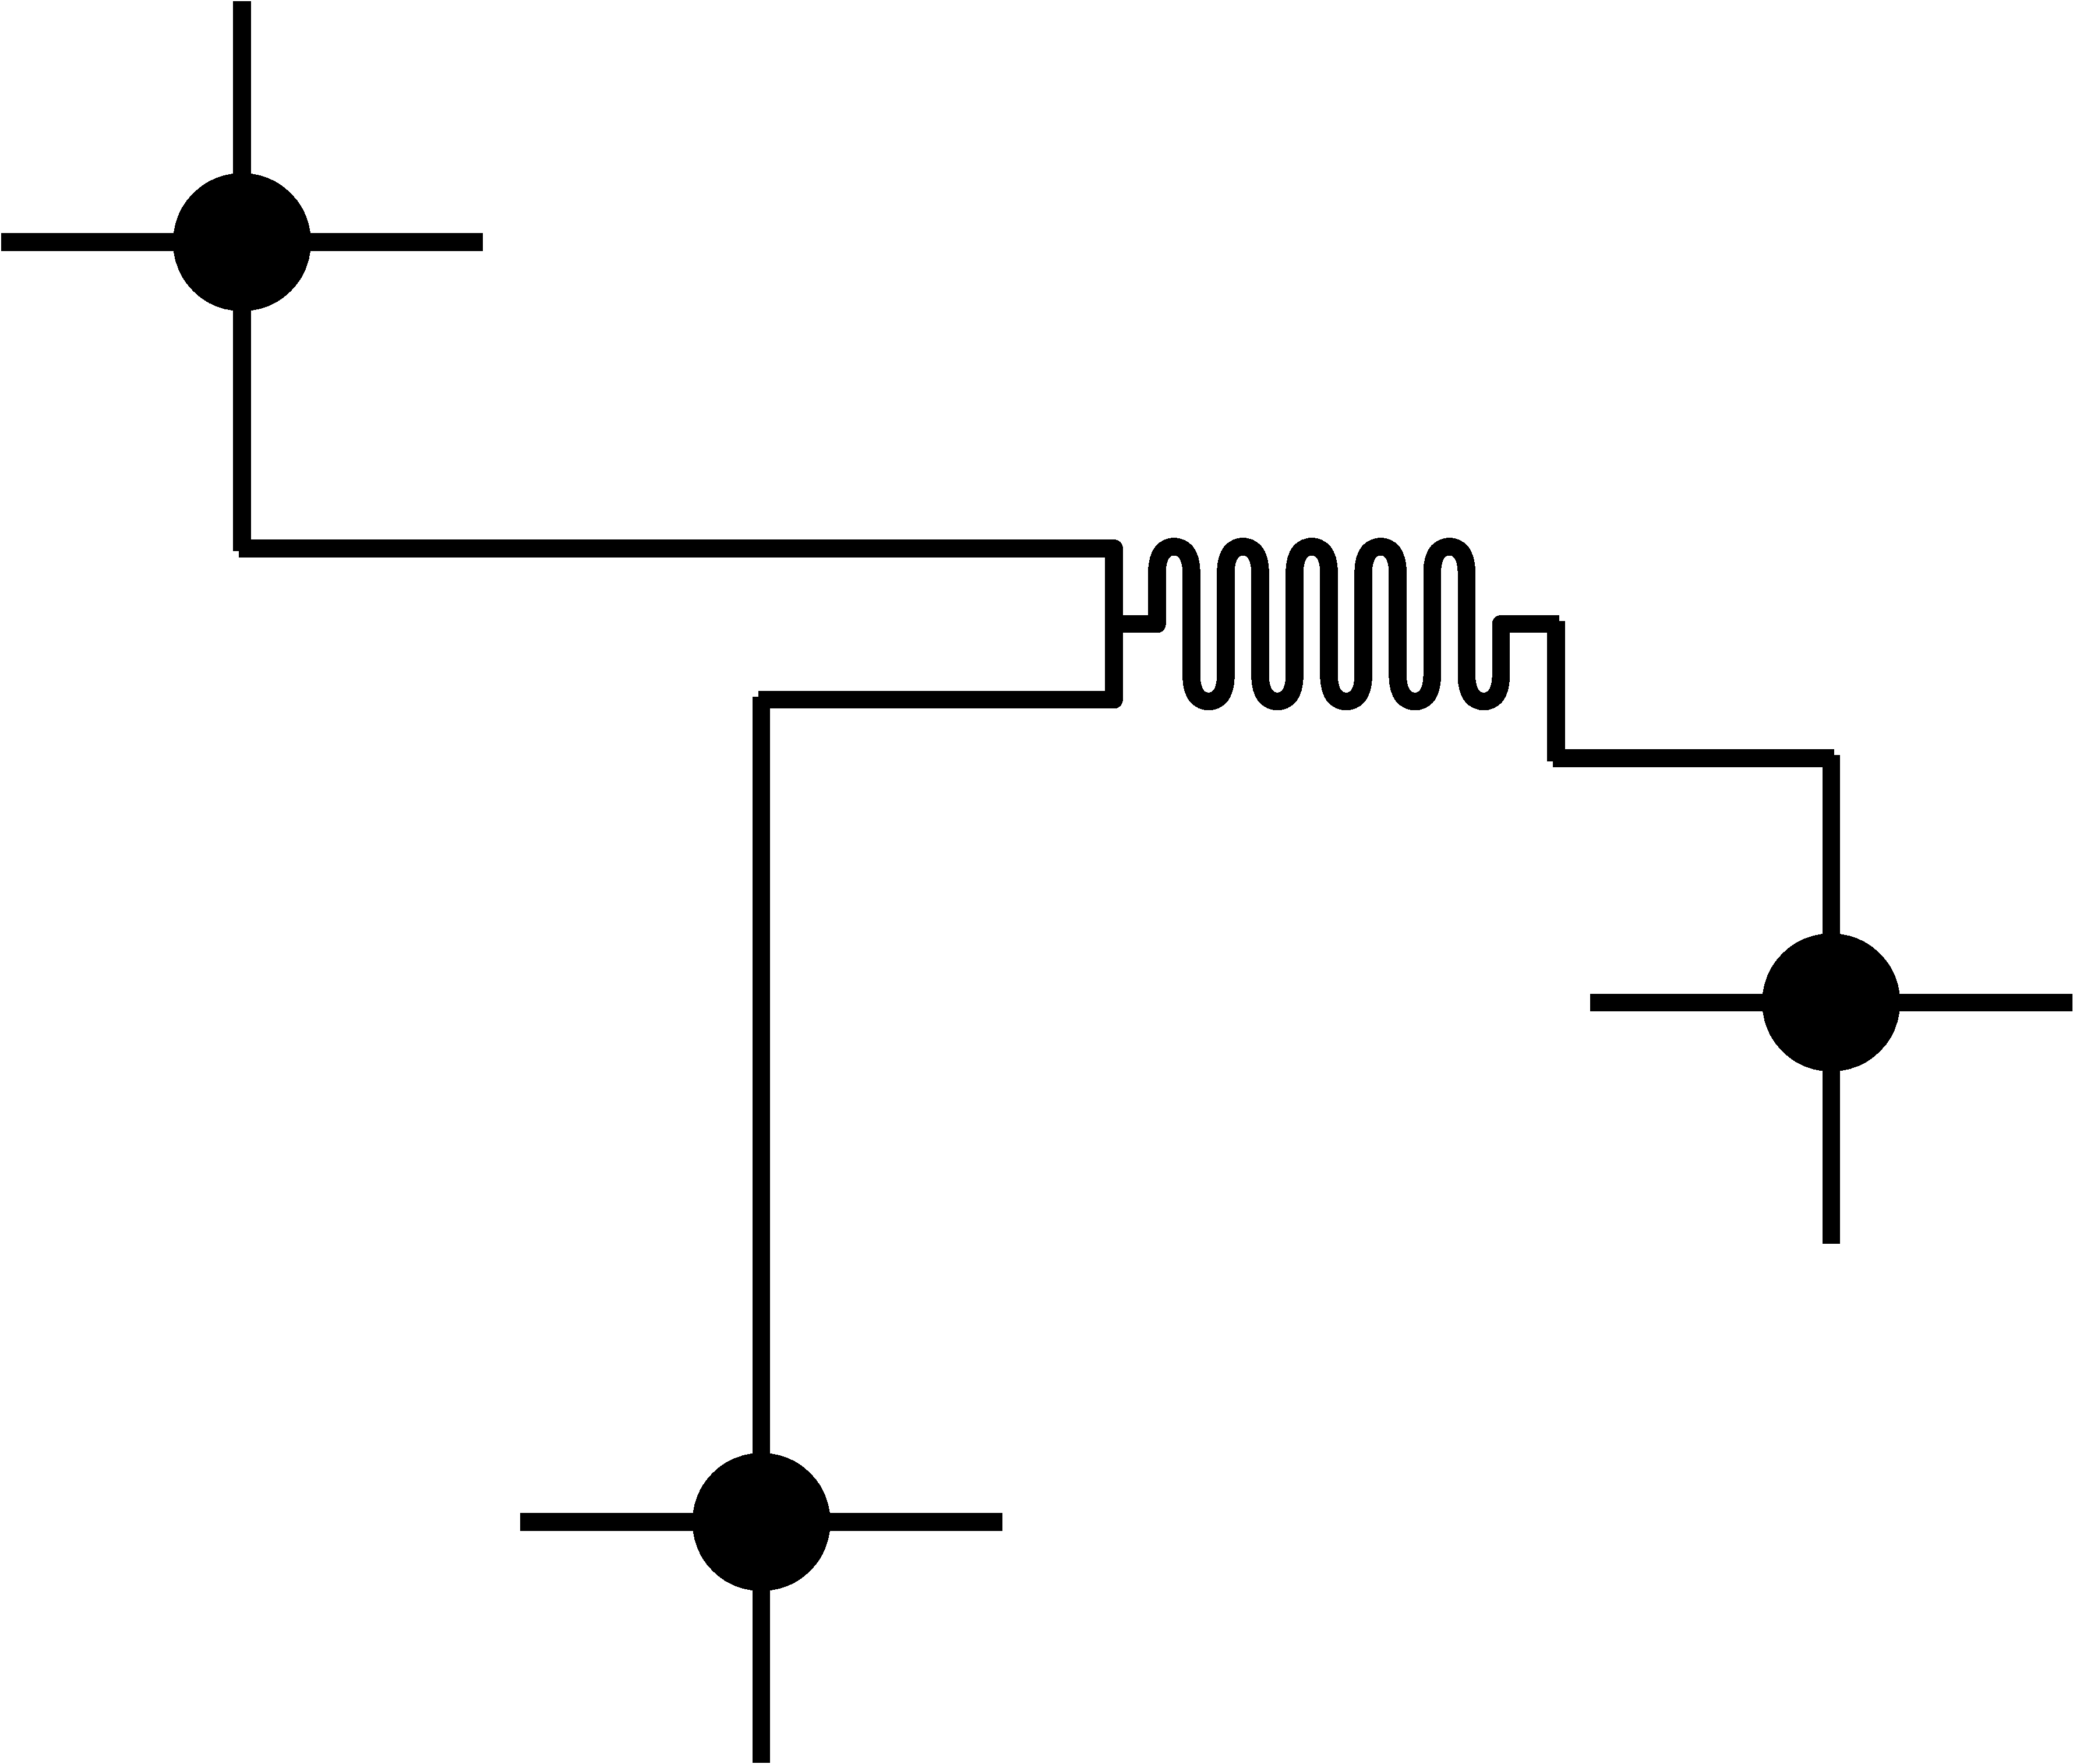
\includegraphics[width=0.9\textwidth]{figures/synthesis_process_routing.pdf}}
        \caption[short]{}
        \label{fig:routing}
    \end{subfigure}
    \begin{subfigure}{0.33\textwidth}
        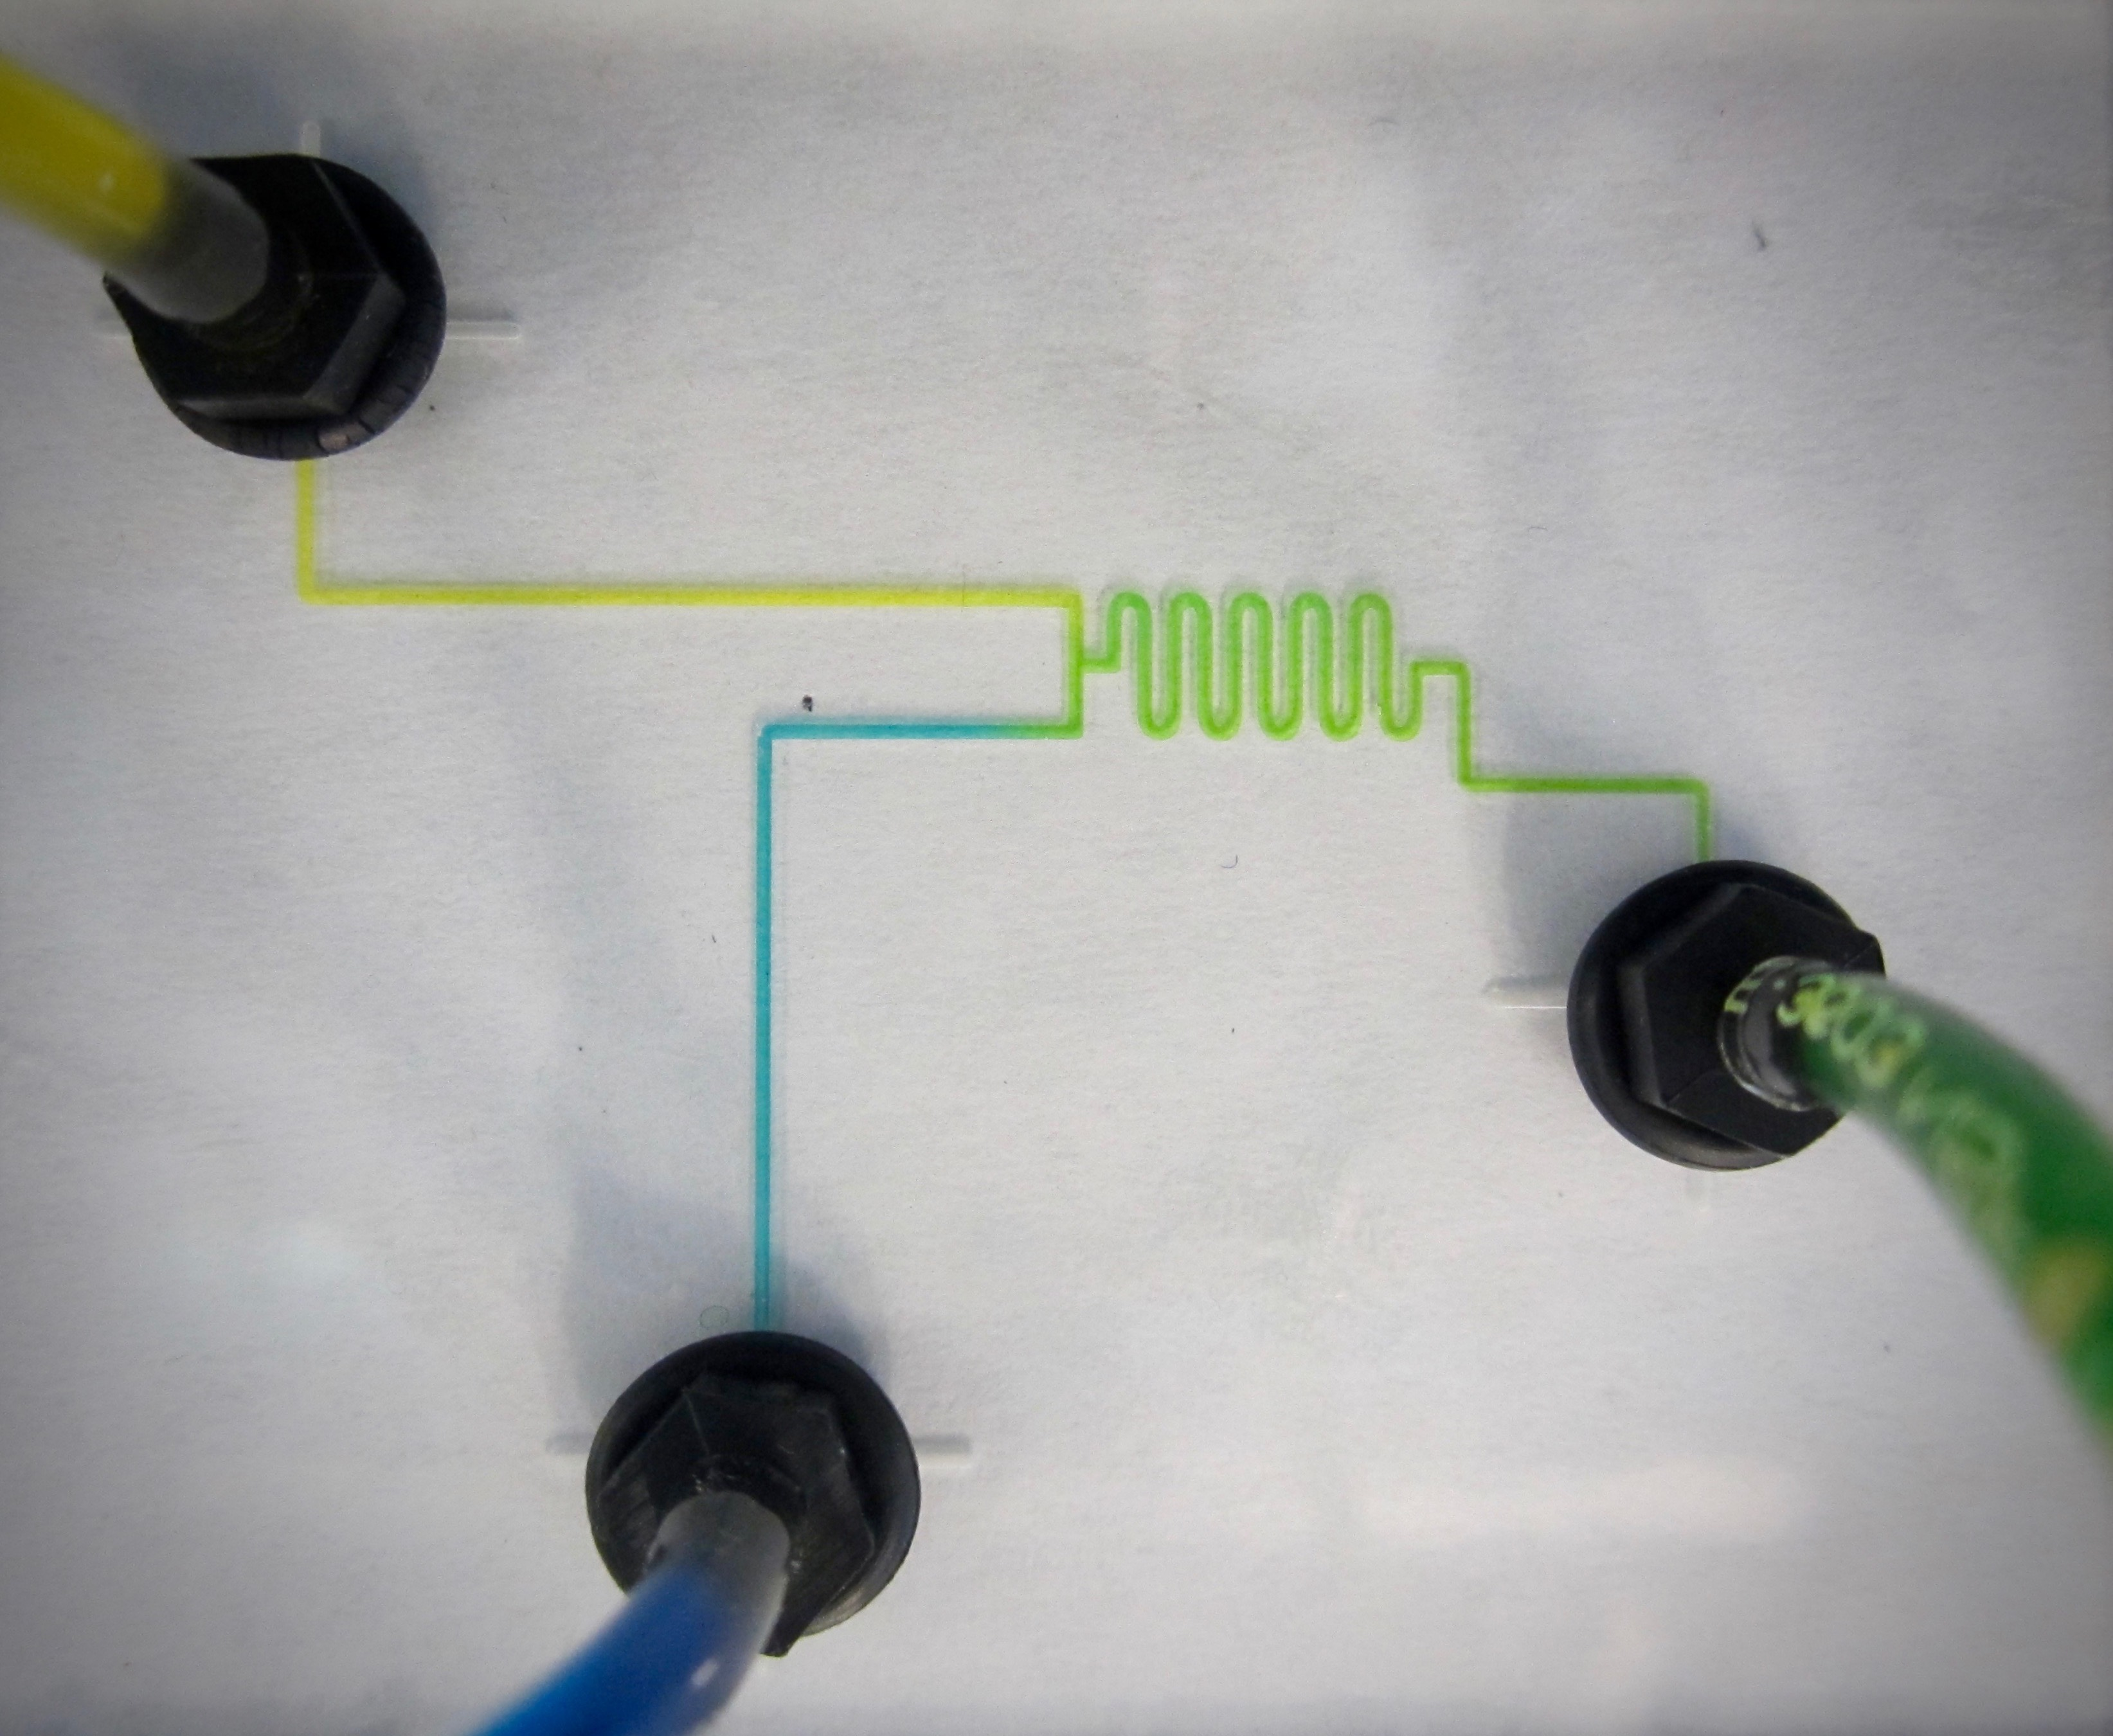
\includegraphics[width=0.97\textwidth]{figures/synthesized_mixer.jpg}
        \caption[short]{}
        \label{fig:fabricated_chip}
    \end{subfigure}
    \caption{Fabricating a flow-based devices begins with a \bs{} program (\cref{fig:bs_program}).  In \cref{fig:net_list} the \bs{} compiler then generates the components and connections (netlist).  A synthesis tool will then attempt to place the components on a device\Cref{fig:placement} and further attempts to route the connections prescribed in the netlist\cref{fig:routing}.  If both placement and routing are successful, the device can be fabricated (\cref{fig:fabricated_chip}) using any of the fabrication processes currently used.}
    \label{fig:synthesis_process}
\end{figure*}
%=================================================================================
% Experimental
%=================================================================================
\section{Experimental}
\label{sec:experimental}
The architecture of \tool{}, as depicted in \cref{fig:workflow}, amounts to the experimental setup.
It is comprised of extending and integrating \bs{} with Inkwell in order to include support for (1) targeting Inkwell, (2) component selection, (3) device fabrication, and (4) execution.

%=================================================================================
% BioScript
%=================================================================================
\subsection{\bs{}}
\label{sec:bioscript}

We extend the \bs{} compiler, (1) in \cref{fig:workflow}, with the ability to target continuous flow devices.
This amounts to extending the available targets to include an Inkwell\cite{mcdaniel2018design} target.
Part of this extension includes: component selection, ParchMint generation, and, optionally building a valve actuation sequence.
In component selection, the target selects the best component that matches the function of the operation.
For instance, given the instruction in line 7 of \cref{fig:bs_program}, the target will pick a serpentine or circular mixer for passive and active flow devices, respectively.
It is parameterized such that if a time definition exists on the $\textsf{mix}$ instruction, component selection will attempt to select the best match; opting to round up when necessary.\footnote{We acknowledge that without additional knowledge of the properties of the fluids (e.g. density, viscosity), a `best match' mixing component may not be appropriate to achieve homogeneity between the operands.}
Once components are selected, the compiler builds the connections between these components as a netlist (\cref{fig:net_list}).
A connection is defined as a via between a component that \textit{defines} a variable\footnote{A variable is defined when it appears on the \textit{left}-hand side of a statement, e.g., $a = 3$, $a$ is defined as $3$.} and any \textit{uses}\footnote{A usage of a variable is when a variable appears on the \textit{right}-hand side of a statement, e.g., $b = a + 3$. Where $a$ is being used in a statement, but not defined.}.
If the target device is an active-flow device, the compiler will further generate the valve actuation sequence required to actuate the necessary valves on the device for pumping the fluid(s) through the device.
Once \bs{} finishes compilation, the netlist is sent to Inkwell to begin the fabrication process.
\jasoni{From Brian: We should cite the ParchMint format here (and perhaps include a link to the website/github) since I don't think its mentioned anywhere else as the interchange format.}


%=================================================================================
% Inkwell
%=================================================================================
\subsection{Inkwell}
\label{sec:inkwell}

% After \bs{} has converted the high-level language assay into a netlist it needs to be placed and routed to generate a design for fabrication.
The input netlist contains a number of components and connections between them, however it does not specify where each component will be located on the device or what route each connection will take to physically connect two components via their ports. Inkwell is an highly extensible system takes a netlist as input and performs placement, routing, and pre/post-processing steps to both the flow and control layer as necessary to generate a design for fabrication. Each step of the process is designed to be modular so new algorithms and process can be introduced, and a ParchMint file can be ingested or generated at any point in the process to allow Inkwell to work in concert with other tools. For this experiment the planar placement and routing method was used with no pre/post-processing steps \cite{mcdaniel2015flow}.

\jasoni{From Brian: I'm not sure how much we want to talk about Inkwell specifically here so I left it pretty general and short (if we have some more room I would love to dump a bunch of self citations here such as DICE and Seam Carving). I also wasn't sure what to call this step (architectural synthesis I don't think is appropriate in this case) which I think makes it read a bit weird. }

%=================================================================================
% Component Selection
%=================================================================================
\subsection{Component Selection \& Generation}
\label{sec:component_selection}

As discussed in \cref{sec:synthesis}, component selection isn't an active area of research.
In order for \tool{} to correctly map \bs{} instructions to their corresponding component, \tool{} employs a naive solution, relying upon a simple mapping of pre-generated components.
This naive implementation is flexible enough to demonstrate efficacy of \tool{} while still maintaining fidelity with commonly utilized assays.
However, we recognize that \tool{} is currently not capable of capturing the true nuances of fluids and how they behave flowing through their selected components.
\briani{Do we plan on addressing this in the future?}

%=================================================================================
% Assay Execution
%=================================================================================
\subsection{Device Fabrication \& Assay Execution}
\label{sec:assay_execution}

All devices, whether generated by hand or using \tool{}, require a domain-expert to ``validate'' the design.
Since \bs{} nor the netlist do not account for physical attributes of fluids, this step is still necessary.
A domain expert must ensure the geometries, channel widths, etc. are correct with respect to the specification and that the device will operate relative to fluidic attributes.
We expect, through component generation, even if naive, to reduce this burden.
However, because Inkwell generates an SVG\jason{give the acronym if Brian hasn't talked about it in \cref{sec:inkwell}}, there is no real time investment for a domain expert.
The SVG, in this context, is then sent to Computer-Aided Design (CAD) software, where the device can then be fabricated using any of the techniques mentioned above.

In practice, this experiment uses a CNC mill to mill a negative in acrylic.
We then bond a glass layer to the acrylic layer.
Once the bond has cured, I/O ports are then connected to their respective reservoirs and the device is ready to be used.
The devices are capable of either being powered by gravity or, as in our case, external syringe pumps.
%=================================================================================
% Results and Discussion
%=================================================================================
\section{Results \& Discussion}
\label{sec:results_discussion}

We measured the time it took to program an assay and synthesize a corresponding device.
These assays are arbitrary in purpose; only including primitive operations (\textsf{mix}, \textsf{split}, \textsf{detect}, \textsf{heat}, and \textsf{dispose}/\textsf{dispense}).
For the purposes of these experiments we assume simple components, e.g., all detection modules behave the same in form (one input, one output), or splits can only split into some power of 2 ($2^n$).
Our intent is to demonstrate the efficacy of the workflow in its entirety, not highlight the features or limitations of any of the discrete tools used in this workflow or demonstrate a new or novel way to handle component selection or generation.
Similarly, our experimental setup does not include the time taken to fabricate or execute the device as the fabrication of the device is dependent upon too many variables: the placement and routing algorithms used to synthesize the device, the actual device fabrication technique (photo-lithography, CNC mill, etc), or what type of device is being fabricated (continuous or active flow) in addition to assembly and setup.

We generated \cref{tab:synthesis_time} using a 2.7 GHz Intel\texttrademark Core i7 processor, 8GB RAM, machine running macOS\texttrademark.
To test the efficacy of \tool{}, we create various assays of increasing complexity as presented in \cref{tab:synthesis_time}.
By leveraging \tool{}, we are capable of creating assays comprised of 50\footnote{A restriction in the way Inkwell handles placement and routing of components limits experimentation to 50.  A limitation that is currently being remedied, but not yet complete.} components in \jason{add time}.
We acknowledge that these results are in a vacuum --- free from comparison of how traditional microfluidic devices are created.
We have been unable to find any quantitative information regarding the time required to design and fabricate these devices.

\begin{table*}[htb]
\centering
\caption{Results demonstrating the time it takes to express an assay (using \bs{}) and then synthesize the corresponding device (using Inkwell).  The results clearly demonstrate how well this workflow performs at building successively more complicated devices; a task that, when done by hand is exceedingly arduous and onerous.\jasoni{add times}}
\label{tab:synthesis_time}
\begin{tabular}{@{}rrrrr@{}}
\toprule
Number of & \bs{} Time & Compilation Time & Synthesis Time & Total Time \\
Components & (mm:ss) & (ss.ms) & (hh:mm:ss) & (hh:mm:ss) \\ \midrule
4 & 00:26 & 0.2448 & 00:00:00 & 00:00:00\\
6 & 00:45 & 0.2457 & 00:00:00 & 00:00:00\\
16 & 02:48 & 0.2700 & 00:00:00 & 00:00:00\\
24 & 03:03 & 0.2845 & 00:00:00 & 00:00:00\\
50 & 06:49 & 0.3506 & 00:00:00 & 00:00:00 \\ 
100 & 12:36 & 0.4226 & 00:00:00 & 00:00:00 \\
1000 & 102:09 & 1.3520 & 00:00:00 & 00:00:00 \\
\hline
\end{tabular}
\end{table*}

Having demonstrated how we tested \tool{}, we now analyse and discuss the results of our experimentation.
\tool{} is the first workflow of it's kind, capable of quickly and efficiently synthesizing assays of complexities far greater than what current practices allow.
It is important to note that \tool{} does not track fluidic or device properties such as: fluid viscosity, fluid density, channel resistance, or length.
This necessitates a domain expert to validate a design and make any modifications necessary to fabricate a functional device.
Reducing the load of a scientist from manually placing and routing each component to quickly validating a device mask greatly reduces the time between assay expression and assay execution.
A problem further discusses in \cref{sec:conclusion}.

% \textit{This is arguably the most important section of your article.}

% \textit{Your results should be organised into an orderly and logical sequence. Only the most relevant results should be described in the text; to highlight the most important points. Figures, tables, and equations should be used for purposes of clarity and brevity. Data should not be reproduced in more than one form, for example in both figures and tables, without good reason.}

% \textit{The purpose of the discussion is to explain the meaning of your results and why they are important. You should state the impact of your results compared with recent work and relate it back to the problem or question you posed in your introduction. Ensure claims are backed up by evidence and explain any complex arguments.}
%=================================================================================
% Conclusion
%=================================================================================
% This is for interpretation of the key results and to highlight the novelty and significance of the work. The conclusions should not summarise information already present in the article or abstract. Plans for relevant future work can also be included.

\section{Conclusion}
\label{sec:conclusion}

We have both provided and demonstrated a grand vision for the future of design and fabrication of flow-based microfluidic devices.
This vision prescribes a fundamental change in the way flow-based assays are currently expressed and then fabricated; relying on an automated synthesis framework to allow for increasingly complex devices.
This vision is not perfect nor complete, but makes significant tangible progress aiming to reduce the perpetual ``5 year'' promise of radical transformation.
There are many outstanding questions requiring answers to further this vision, but are outside the scope of this paper.

%=================================================================================
% Future Work
%=================================================================================
%\subsection{Future Work}
%\label{sec:future_work}
One orthogonal research avenue would be exploring component reuse and reduction.
Current devices are not large, spatially; however, they can be comprised of dozens of components.
Designing these devices doesn't explicitly identify components capable of reuse.
Automatically detecting and reducing components can reduce design and fabrication time.
Further, component reuse could allow an otherwise unfabricatable device to be fabricated.
This avenue is only possible in active flow devices, as fluid may be flowing backwards through the device.

As noted in \cref{sec:results_discussion}, fluidic properties (e.g., viscosity, concentration, or density) are not captured in the front-end (BioScript) or utilized during device synthesis (Inkwell).
By capturing these properties, \tool{} could further reduce the need for expertise required in fabricating and verifying more interesting and complicated devices.
One interesting application of including fluidic properties is solute separation -- making separating blood cells and cancer cells significantly simpler while using far less blood.
Including these properties has implications for the inclusion of timing constraints as well.
Timing constraints allow a user to specify that a particular fluidic variable must be used within a particular time interval.

Inclusion of fluidic properties would directly influence component generation and selection.
The compiler and synthesis tools can take fluidic properties and make decisions during component generation or selection to deliver the best device possible; manipulating channel width or geometries, influencing placement and routing, or even simply selecting the best component for the fluid.

Finally, extending the compiler to include active-flow devices, devices that use pumps to move fluid through the channels, instead of back pressure or gravity, would be a natural extension; allowing active control of the device --- the ability to change execution based on various readings or inputs.
This would require a further extension to all 4 steps denoted in \cref{fig:workflow}.
Component selection and generation would need to include components that are able to be controlled.
The compiler would need to know how the selected components behave, and how to actuate them.
Fabricating a device with multiple layers is feasible; however, still requires some fashion of human intervention.
The different layers would have to be aligned precisely so they can be bonded.
This step, in using the cost-effective CNC mill, requires human intervention.
Execution of the assay would require a feedback loop that can notify the compiler of any changes to execution.

%=================================================================================
% Conflicts of Interest
%=================================================================================
\section{Conflicts of Interest}
\label{sec:conflicts_of_interest}

In accordance with our policy on Conflicts of interest please ensure that a conflicts of interest statement is included in your manuscript here.  Please note that this statement is required for all submitted manuscripts.  If no conflicts exist, please state that ‘There are no conflicts to declare’.

%=================================================================================
% Acknowledgements
%=================================================================================
\section{Acknowledgements}
\label{sec:acknowledgements}

Contributors (that are not included as co-authors) may be acknowledged; they should be as brief as possible. All sources of funding should be declared.
%%%END OF MAIN TEXT%%%



%The \balance command can be used to balance the columns on the final page if desired. It should be placed anywhere within the first column of the last page.

%\balance

%If notes are included in your references you can change the title from 'References' to 'Notes and references' using the following command:
%\renewcommand\refname{Notes and references}

%%%REFERENCES%%%
\bibliography{references} %You need to replace "rsc" on this line with the name of your .bib file
\bibliographystyle{rsc} %the RSC's .bst file

\end{document}